\chapter{Reproduction experiments}
\label{chap:implementation}

\section{Overview}

In this chapter we discuss the process of building our Deep Reinforcement Learning based query reformulation system, based on the framework proposed by Nogueira \& Cho \cite{nogueira2017task}. This process consists of two phases, in the first phase we set out to reproduce a query reformulation system based on published descriptions from Nogueira \&Cho.The performance of the preliminary experiments suggests that the resulting system may be sub-optimal, as we did not get similar results as them. In order to improve the performance of the system, we set out to find additional implementation information, contacting one of the authors, Nogueira, directly. Valuable insight was gained in this process and we were able to produce an improved implementation.



\section{Reproducing experiments from  Nogueira \& Cho's framework}


The first iteration of our deep reinforcement learning based query reformulation system is implemented based on our interpretation of the algorithms and parameters provided by Nogueira \& Cho\cite{nogueira2017task}. By following the implementation and parameters presented in the paper itself, we are motivated by the goal to confirm that the mechanism described in the paper is complete, to gather further insight on the working of the system, and to gain a deeper understanding for the nature of the problem in order to identify ways we can expand this piece of research.

This implementation is based on the theoretical components described in the previous chapter. However, even given the same theoretical framework, details in implementation could make a substantial difference to the experiment results. We take special care to discuss these ambiguity and describe our design decisions.

\subsection{Interpreting input of the model}

Nogueira \& Cho \cite{nogueira2017task} described the inputs to the model as follows: \newline

\textit{``The inputs are a query $q_0$ consisting of a sequence
of words ($w_1$, ..., $w_n$) and a candidate term
$t_i$ with some context words ($t_{i-k}$, ..., $t_{i+k}$), where
$k$ $\geq$ 0 is the context window size. Candidate terms are from $q_0 \cup D_0$, the union of the terms in the original query and those from the documents $D_0$ retrieved using $q_0$. We use a dictionary of pretrained word embeddings to convert the symbolic terms $w_j$ and $t_i$ to their vector representations $v_j$ and $e_i \in \mathbb{R}^{d}$ , respectively.
''} \newline

From this description we can identify that there are two inputs to the model.

\begin{itemize}
\item $q_0$, the original query we wish to reformulate. $q_0$ contains a set of terms ($w_1$, ..., $w_n$)	
\item $t_i$, a single instance of a candidate term, along with some number of neighbouring terms on each side of it to provide contextual information.
\end{itemize}



The first input, the raw query  $q_0$, is the query we wish to reformulate, acquired from the user. 

The second input, candidate term $t_i$  are from documents retrieved by an initial round of search operation. During this first round of search the raw query $q_0$ is sent to the search engine, which returns a ranked set of documents, $D'$, containing documents considered to be relevant with regard to the raw query, $q_0$. 
\begin{figure}
	\centering
	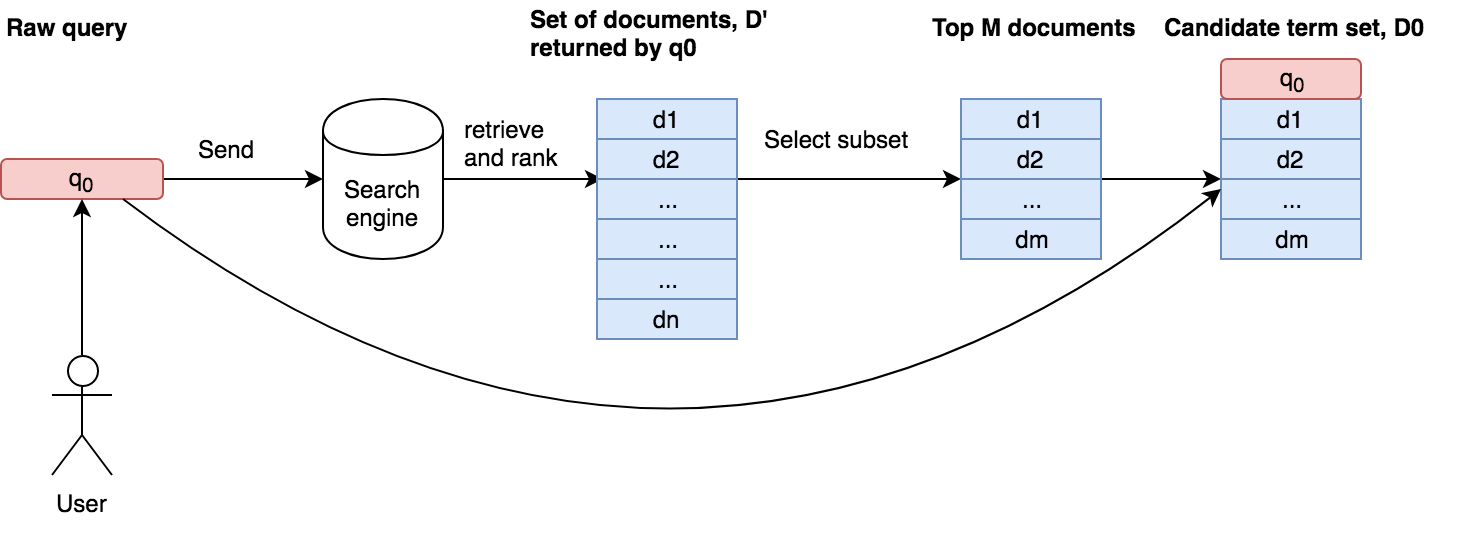
\includegraphics[width=1\textwidth]{images/chapter_4/Chapter_4-source_of_candidate_terms.png}
	\caption{The process of sourcing candidate terms}
	\label{fig:cand_source}
\end{figure}
From this set of documents, a subset, $D_0$, likely to be the top $M$ documents in this ranked results list, are selected as candidate term source. The value of $M$ is a parameter which we experiment with in our preliminary experiments. As Noguiera \& Cho state that candidate terms are from $q_0 \cup D_0$, we treat $q_0$ as an individual document for the purpose of selecting candidate terms, and append it to the list of documents in $D_0$, this is the set of documents where each candidate term $t_i$  is sourced from.  The process of generating a set of candidate terms from the raw query is illustrated in figure \ref{fig:cand_source}.



\subsubsection{Context window}

In the description provided above, Nogueira \& Cho\cite{nogueira2017task} addresses the use of $k$ context terms alongside each candidate term, $t_i$, stating this design is highly important, because it captures the contextual information about the candidate term. 

We interpret this description as moving a sliding window of size $2k + 1$ through each candidate document and producing ``slices'' of the candidate document. Where each instance of the sliding window contains the candidate term,$t_i$, in the middle, and $k$ context terms are included on each side of the candidate terms. Special care is taken where the number of context terms available are less than the size of $k$. This can happen when the current candidate term, $t_i$ is near the boundaries of an document, or when the document contains less than $2k + 1$ terms (this is likely the case when we treat the original raw query as another document). In these circumstances, we used a special token to pad out such document. 

For example, suppose a raw query is ``the ultimate answer'' and the document is ``the answer to life the universe and everything is 42'', and the number of context terms, $k$, is 1, this is equal to moving a sliding window of size 3 through the document and capturing each ``slice'' of document as a tri-gram.  Figure \ref{fig:chapter4-contextwindow} illustrates this process, the candidate term in each slice is in bold, note that at the edges of the document a special token is used for padding.

\begin{figure}[h]
	\centering
	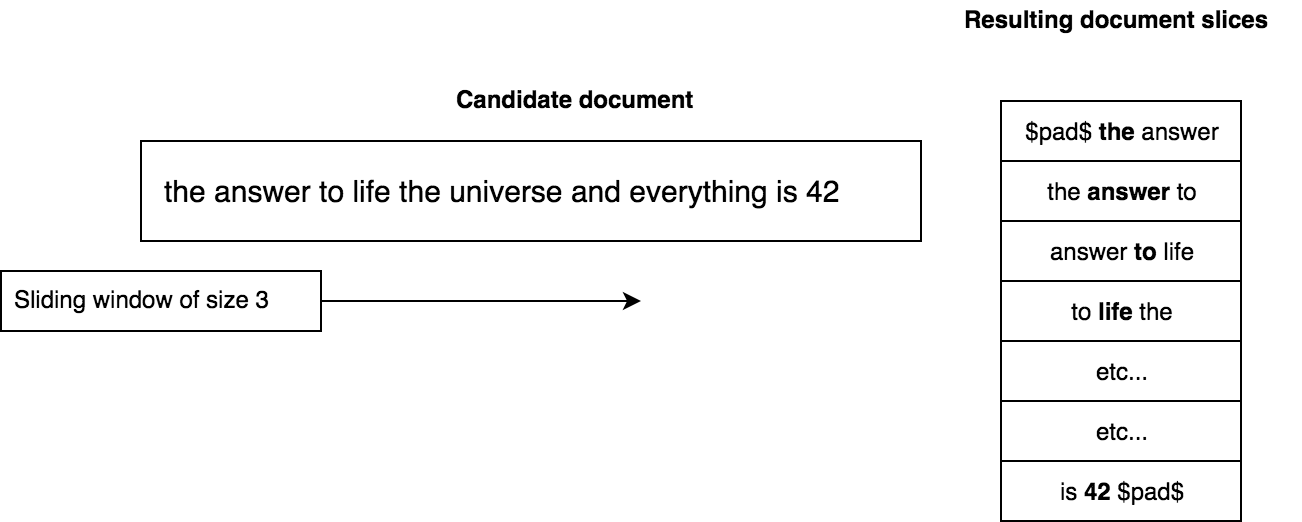
\includegraphics[width=1\linewidth]{images/chapter_4/Chapter_4-context_window}
	\caption{Illustration of using a sliding window to each candidate term with context term from the document.Candidate term is in bold}
	\label{fig:chapter4-contextwindow}
\end{figure}


After acquiring ``slices'' of all candidate documents, each candidate term as well as terms in the raw query is converted from natural language into their Word2Vec embedded vector representation with a dictionary look up, using a pretrained Word2vec embeddings. The special token used for padding edges of document are converted into padding vectors where all dimensions are set to 0.



\subsection{Feature extraction using convolutional neural network}

Nogueira \& Cho \cite{nogueira2017task} described the use of convolutional neural network to obtain a “fixed size vector representation” for the entire sequence on the query side of the input, and for each term in the candidate side of the input. The description is provided as such: 

\textit{``We convert the sequence $v_j$ to a fixed-size vector $\phi_a(v)$ by using a convolutional neural network (CNN) followed by a max pooling operation over the entire sequence. Similarly, we fed the candidate term vectors $e_i$ to a CNN to obtain a vector representation $\phi_b (e_i)$ for each term $t_i$. ''}

On the architecture of their Convolutional Neural Network, Nogueira \& Cho \cite{nogueira2017task} reported:

\textit{``We use a 2-layer convolutional network
for the original query. Each layer has a window
size of 3 and 256 filters. We use a 2-layer convolutional
network for candidate terms with window
sizes of 9 and 3, respectively, and 256 filters
in each layer.''}

\subsubsection{2-layer CNN}

From the descriptions above we interpret that there are two separate convolutional neural networks. One to process the original query, taking the vector representation(Word2Vec embedded vectors) of the entire raw query as the input; one for the candidate terms, taking the vector representation of each candidate term, along with their context terms as input, and there are two layers for each CNN model.

We interpret the window size specified as the width of each filter. Because the input to the CNN are Word2vec embedded vectors,  where each vector represents a whole term and cannot be viewed partially,the length of the CNN filter must match with the length of the term vectors. The width of the filters correspond to the number of input terms processed at each step.  Multiple filters are used because each filter is initialised with different weights, thus each filter will capture a different features from the input. Conceptually, it is somewhat analogous to the idea of a pair of human eyes looking at an image with glasses of various shades.  

In figure \ref{fig:CNN2} we illustrate this process using a trivial example.  In this illustration, 5 filters are used to process some input text in the format of word2vec embeddings, the height of the input is the number of dimensions used to embed each term, and the width of the input is the number of terms in this input phrase, let this number be 9 (so there is one candidate term in the centre, with 4 context terms on either side). 

The filters have the same height as the input, and a width of 3. Assuming the filters pass through every input term (using padding around the edges of the input), at each stride through the input the filter would produce a single number representing the feature captured. After completing a pass through the input, each filter would produce a feature vector of size $len(input)$. Combining these feature vectors would result in a feature map. In this example, a feature map of size $5 \times 9$ is produced because there are 5 filters, and the input phrase is 9 terms long.




\begin{figure}[H]
  \centering
    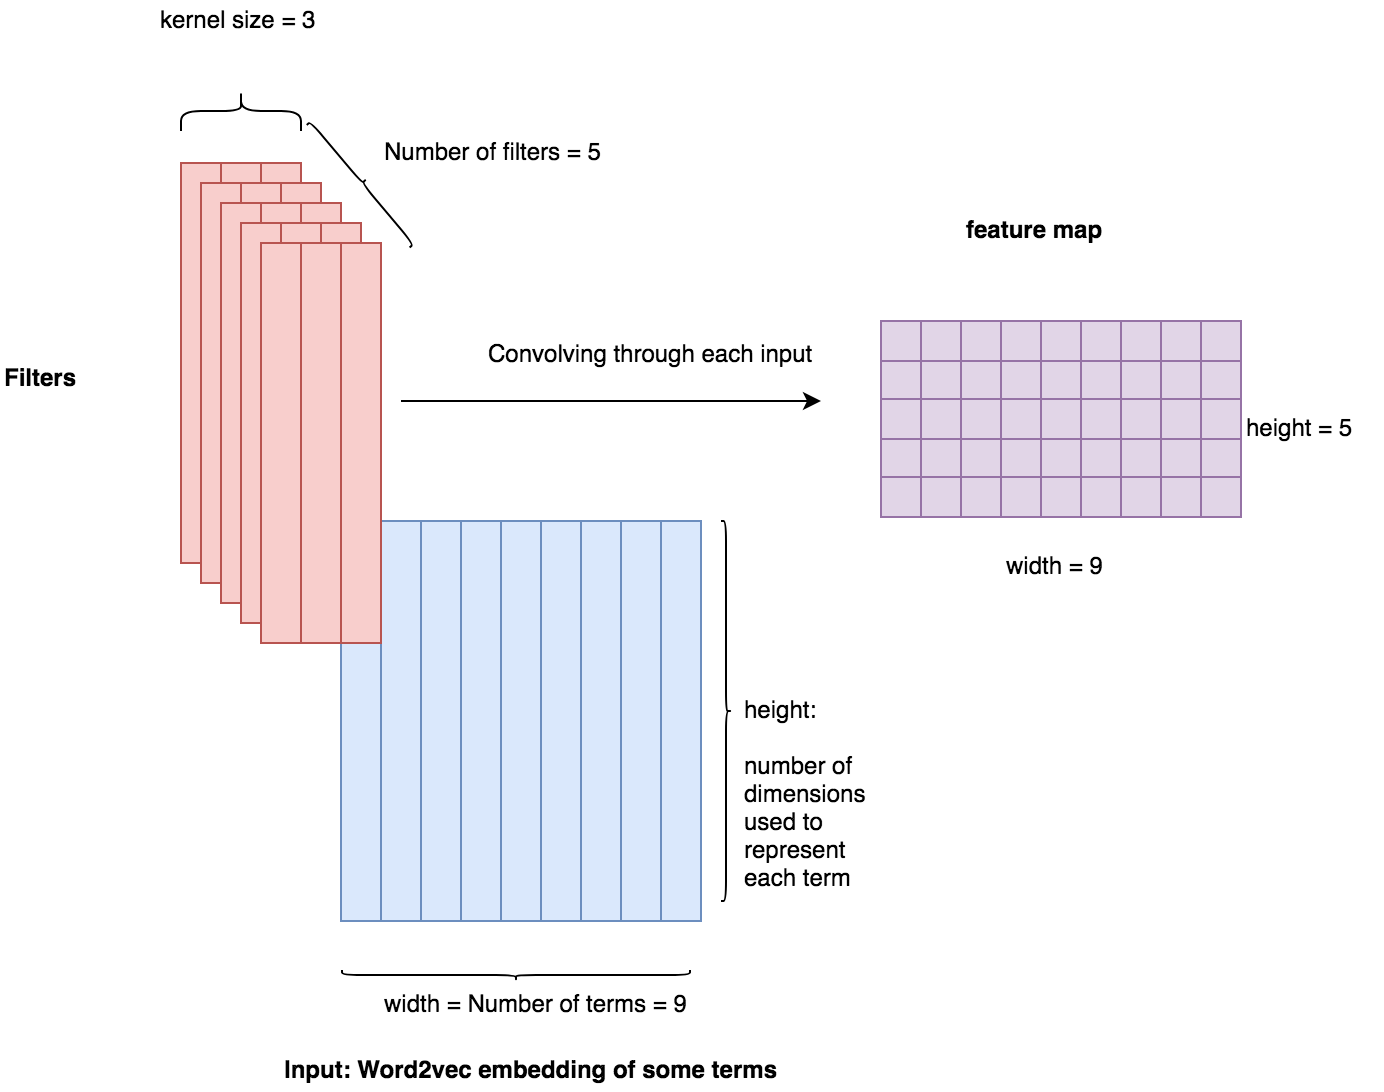
\includegraphics[width=1\textwidth]{images/chapter_4/Chapter_4-CNN2.png}
    
  \caption{Feature extraction from embedded input text using convolutional filters}
    \label{fig:CNN2}
\end{figure}


The input goes through two layers of convolution operation similar to the illustration in figure \ref{fig:CNN2} , taking the output of the previous layer as input to the next layer. After this, a max pooling operation is performed to extract the ``fixed size vector'' representation of the input texts. 

These steps are performed on the raw query, as well as each candidate term.   Figure \ref{fig:CNN1} illustrates this architecture. In this example, the raw query is ``South African Sanctions'', from the WSJ dataset, and the candidate term to be assessed for suitability is ``apartheid'', from a document about the Anti-Apartheid act retrieved by the initial round of search. The candidate term has one neighbouring context term on either side of it. These inputs gets processed with their separate 2-layer CNN, resulting in a fixed sized vector for the input query and a fixed sized vector for the combination of candidate and context terms.These two vectors are combined and passed onto the policy and value network for prediction.

\begin{figure}[H]
	\centering
	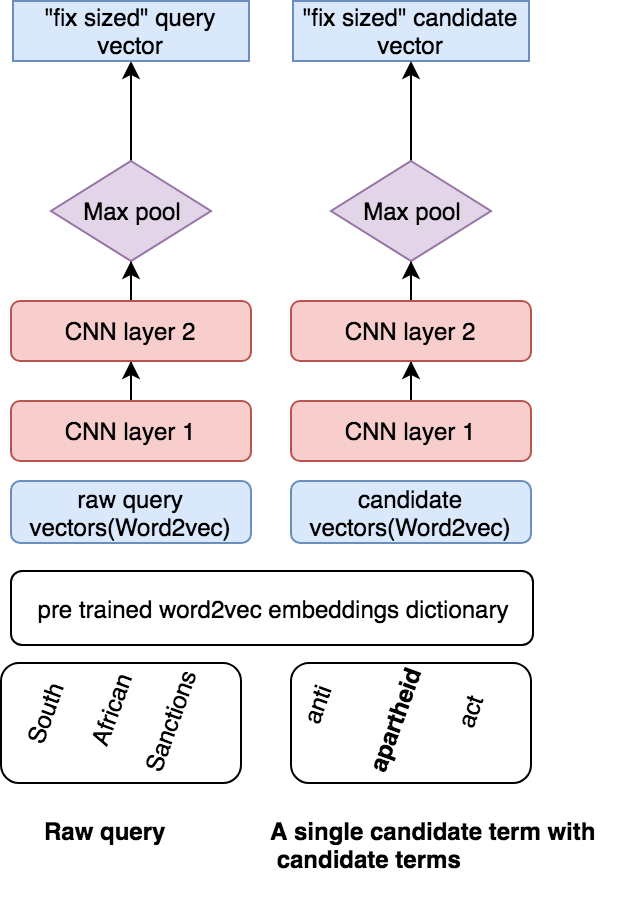
\includegraphics[width=0.7\textwidth]{images/chapter_4/Chapter_4-CNN.png}
	\caption{An illustration of the hierarchical CNN architecture}
	\label{fig:CNN1}
\end{figure}



\subsection{Policy and value networks}

Following the two CNN layers, a policy predictor and a value predictor, both fully connected neural networks are used to generate the final outputs of the model. The policy network predicts the raw probability that the candidate term should be included in the reformulated query, the value network predicts the expected reward attainable from the current state.

The role of the policy predictor is to predict whether a term should be used to rewrite the query. Nogueira \& Cho\cite{nogueira2017task} interprets the output of the policy network as the raw probability that a term should be used to rewrite the query, stating that :

\textit{``We compute the probability of selecting $t_i$ as:}
% \begin{equation}
%     (R - \bar{R}) - \sum_{t_i \in T} log(ti|T) 
% \end{equation}
\begin{equation}
P(t_i|q_0) = \sigma(U^T tanh(W(\phi_a(v)|| \phi_b(e_i)) + b))
\end{equation}

\textit{Where $\sigma$ is the sigmoid function, $||$ is the vector concatenation operation, $W \in \mathbb{R}^{d\times2d}$  and $U \in \mathbb{R}^d$ are weights, and $b \in \mathbb{R}$ is a bias. ''}

This description is relatively straight forward, we interpret this as concatenating the “fixed size vector representation” of the raw query and the “fixed sized vector” representation of a candidate term. This combined vector passes through two layers of fully connected neural network, the first of the layers use a hyperbolic tangent activation function with a bias value, the final layer uses a sigmoid function with no bias value. For each candidate term, the model would generate an output between 0 and 1, we interpret this as the raw probability to include this term in the reformulated query. 

This score is sampled to produce a binary decision on the inclusion of the current candidate term in the reformulated query.

\begin{figure}
  \centering
    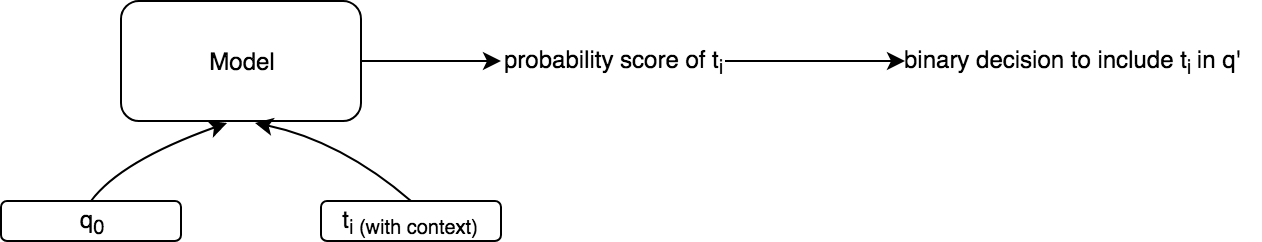
\includegraphics[width=1\textwidth]{images/chapter_4/Chapter_4-term_selection_process.png}
  \caption{An abstract view of the decision making process}
    \label{fig:CNN1}
\end{figure}

An interesting implication here is that the selection of a candidate term to form a new query, q’ is independent on whether or not other candidate terms have been selected. In fact, the agent has no way of knowing whether other terms have been selected. The only piece of information available to the learning agent at the time of the decision is the candidate term examined, it's context terms, and the original query. 

Similar to the policy predictor, the value predictor is a two layer fully connected neural network. A value predictor is used to predict the expected reward the agent would receive by sending the current query to the search engine. 

In the context of policy gradient methods, this value is used to reduce the variance in policy estimation. Nogueira \& Cho \cite{nogueira2017task} provided the following description:


\textit{``We compute the probability of selecting $t_i$ as:}

\begin{equation}
\bar{R} = \sigma(S^T tanh(V(\phi_a(v)|| \bar{e})) + b))
\end{equation}

\textit{ $\bar{e}=\frac{1}{N} \sum_{i=1}^{N} \phi_b(e_i), N=|q_0 \cup D_0|, V \in \mathbb{R}^{d\times2d}$ and $S \in \mathbb{R}^d$ are weights, and $b \in \mathbb{R}$ is a bias. ''}


Base on this description, we interpret the network used for value predictor to be approximate identical in architecture to the policy estimator. The input to the value predictor is the concatenation of the fixed size vector representation of the original query along with a fixed sized vector containing the mean value of all candidate terms vectors. This concatenated vector gets passed through two layers of fully connected neural network, identically structured to the policy predictor. The output is interpreted as the expected reward with regard to the current raw query and set of candidate terms.







\subsection{Building and training the system}

Based on the interpretation of the details in the paper outlined above, we built the first iteration of our query reformulation system. 

\subsubsection{Candidate term source}
We source the candidate terms by performing a search operation using the raw query, on the corpus corresponding to the dataset, using ATIRE with BM25 as the ranking function. 

\subsubsection{Training word embeddings}

We trained the Word2vec word embeddings using Gensim, an open source natural language processing tool-kit. There is little formal motivation on choosing the number of dimensions to represent a term. However, empirical evidence in literature suggests that a dimension of 300 will yield accurate results while maintaining a reasonable training time \cite{pennington2014glove}. Based on this suggestion, we set our vector dimension to be 300. 

We train the word embedding using the same corpus the retrieval task is performed on. After training is complete, the trained Word2Vec model is stored on disk in a dictionary structure and loaded into memory when training the reinforcement learning agent. This improves the efficiency of training by reducing the turnaround time per training session. 


\subsubsection{Neural network configuration}
We built the neural network models using Tensorflow. Following the description provided by Nogueira \& Cho\cite{nogueira2017task}, we set up our CNN to have two layers, with 256 filters in each layer. The fully connected layers used for policy prediction and value prediction are a two layer fully connected neural network with 256 nodes in each layer. 


\subsubsection{Optimiser}

We use ADAM \cite{kingma2014adam}, the state of the art in stochastic optimization as the method to minimize the losses, using a learning rate of $10^-5,\alpha=10−4,\beta_1 =0.9,\beta_2 =0.999$,and $\epsilon=10^{-8}$, the default parameters as suggested by Kingma \& Ba in the paper introducing ADAM.

\subsubsection{Loss function}

 The loss function provided by Nogueira \& Cho\cite{nogueira2017task} for the policy agent is based on the REINFORCE algorithm, in this context it is defined as as:

\begin{equation}
    (R - \bar{R}) - \sum_{t_i \in T} log (t_i|q_0) 
\end{equation}

Where $q_0$ is the raw query, T is the reformulated query, R is the true reward received by assessing the reformulated query, and R’ is the predicted reward from the output of the value network. 

This loss function takes each term in the reformulated query and update the agent's parameters, $\theta$ such that the probability score of these terms increases if the reformulation was considered successful. This is defined by the actual reward, $R$ being greater than expected reward, $\bar{R}$. This update makes these terms more likely to be chosen in a reformulated query with regard to $q_0$ in the future. If the query's reward is less than the model's expectation, in the case where $\bar{R} > R$, then the opposite occurs, the weights are adjusted such that the model will generate slightly lower probability score for these terms in the future.

The value predictor’s loss function is the Mean Squared Error between the actual reward and the predicted reward.


%\subsection{Summary}
%\todo{FIll in a summary of the first system, draw a diagram}
%



\section{Preliminary experiments}
Once we built the system based on descriptions provided by Nogueira \& Cho, we conducted several experiments to evaluate the performance of the system. The main purpose of these experiments was to confirm whether our implementation of the system was correct, and to find out the effectiveness of our system compared to the their results. 



\subsection{Experimental configurations}

\subsubsection{Search engine parameters}

The corpus is indexed using ATIRE's standard indexer, which parses and tokenizes the corpus, then stores it into an inverted index. Initial round of retrieval in order to generate candidate terms is performed using ATIRE’s search, using BM25 with default parameters ($k1=0.9,b=0.4$) as the ranking function. 


\subsubsection{Experimental benchmarks}

\begin{itemize}
	\item Raw ATIRE search of the original query, BM25 with default parameters (k1=0.9,b=0.4) as the ranking function. 
	
	\item ATIRE's implementation of Pseudo relevance feedback based on Rocchio's algorithm
\end{itemize}



\subsubsection{Corpus and dataset}

Two sources of data are used to evaluate this implementation of the query reformulation system

\begin{itemize}
	\item \textbf{TREC-WSJ} 
	
	In our experiments we use TREC-WSJ, a standard data set commonly used in ad-hoc retrieval research, described in TREC-3 \cite{harman1995overview}. 
	
	TREC-WSJ  consists of a total of 150 topics, each topic corresponds to a single query which represents the users' information need. The corpus are articles from the Wall Street Journal between the year 1987 to 1992. There are 173252 documents in this collection.
	
	Relevance judgement is provided by human assessors as part of the dataset. Relevance judgements is binary, meaning that a document is either considered relevant with regard to a query, or not relevant.
	
	
	\item \textbf{Microsoft Academic (MSA)}
	
	This is a dataset used by Nogueira \& Cho \cite{nogueira2017task} in their paper. The corpus consists of 480,000 academic articles crawled from Microsoft Academic API, each document containing the title and abstract of a paper.
	
	The retrieval task is slightly different from a standard ad-hoc retrieval task. A query is the name of a paper, and the goal is to find papers cited by the query. This is a challenging task because simply finding terms similar to the original query may not necessarily result in a well performing query.  
	
	As conducting experiments using the entire sets of queries were computationally expensive and time consuming, we select subsets when running preliminary experiments.We subsampled 1000 queries from this dataset and use it for training, validating on 200 queries. 
\end{itemize}


\subsubsection{Evaluation metric}
We used Mean Average Precision(MAP) to measure the effectiveness of the reformulation performed by the agent. Following the description provided by Nogueira \& Cho\cite{nogueira2017task}, we select the value of $K=40$. Keeping measurements uniform helps to evaluate the effectiveness of the system when compared to the published results. 

\subsubsection{Reward to the reinforcement learning agent}

As we wished to directly optimise for improvement of MAP, we used this metric as the reward to the reinforcement learning agent during training. This is a minor point where we diverge from Nogueira \& Cho\cite{nogueira2017task}, who used recall as the reward, but provided little justification in the original paper on why recall is used as a reward when MAP is the metric the authors are interested in, other than the observation that using recall as the reward also increased MAP. 

\subsubsection{Random seed}

We used a fixed seed for random number generation to ensure the experiments will be reproducible. 




\subsection{Query completion}
In the first preliminary experiment we wished to answer a straightforward question, ``In the most trivial scenario, how does the reinforcement learning agent perform at a query reformulation like task”. 

To answer our question, we created a trivial, arbitrary scenario where there is only one query for the agent to reformulate. A query was selected from the TREC-WSJ collection, with a term removed from the raw query such that the performance worsens, and passed to the agent as a raw query. For candidate terms, the agent was presented with the missing term from the original query along with two other noise terms. The purpose of this was to confirm that the reinforcement learning aspect of the model functioned as intended on a small scale problem.


\subsubsection{Conclusion}
This was a trivial problem for the agent, the agent’s policy converged quickly to always selecting the correct term after approximately an hour of training. This confirms that the reinforcement learning aspect of the system is maximizing the reward attainable from the environment. 


\subsection{Reformulating a single query }

In this experiment, we set out to investigate how the agent performed at solving the problem of query reformulation. Once again, we conduct this investigation at a minimal scale. We presented the agent with the task of reformulating a single query from the WSJ collection and observed the reformulation behaviour of the agent over three variants.



\subsubsection{Reformulation using top-10 documents}

In the first variant, we experimented with query reformulation using terms from all documents in the top ten results from the initial round of search using the raw query, the reason is that we did not want to miss any potentially useful term in reformulation. 


\subsubsection{Reformulation using top-1 document, deterministic}

In the second variant, we only use a single document, taken from the top of the results list as a source for candidate terms. The advantage of this is that now the action space has been reduced substantially compared to the first variant. However, there existed a risk that the “perfect term”, which would form the ideal query not being present in the top document. Terms are included in the reformulated query based on the probability output of the policy predictor, we use a greedy approach with a hard threshold for inclusion, if the probability is higher than 0.5, we include the term in the reformulated query, otherwise we discarded the term. 

\subsubsection{Reformulation using top-1 document, adding random noise}

The third variant is set up similarly to the second variant, with an element of randomness added to account for exploration in reinforcement learning. The agent would sample the policy and have a chance of acting in according to the policy output, and a certain probability to act completely randomly, this is controlled by a parameter $e$, initially set at 0.01 and decays as the number of training iteration increases. A random number is generated at the time of agent's decision, if the random number is larger than $e$, then the action would be the agent's policy network's prediction. However, if the random number generated is smaller than $e$, then the final action is based on random chance.  This is known as $e$-greedy, a well-used technique in reinforcement learning \cite{sutton2018reinforcement}.  A reinforcement learning agent acting purely on a greedy policy has a tendency to be stuck in a local optimum. By injecting random noise in the agent’s actions, the agent may do worse in the short term, however, it increases the possibility that the agent would learn a better policy closer to the global optimum.  

\subsubsection{Results}

We train the agent using these three variants over a 24 hour training time, tracking the MAP of the top 40 results compared to the baselines, ATIRE raw search with BM25 as the ranking function, and ATIRE’s pseudo relevance feedback based on Rocchio’s method. The results are shown in figure \ref{fig:reformulated_single_query}.

\begin{figure}[H]
	\centering
	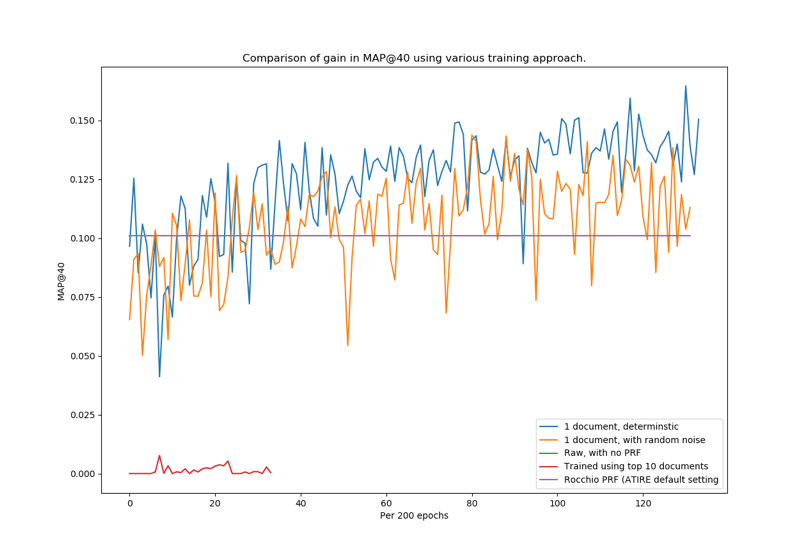
\includegraphics[width=1\textwidth]{images/chapter_4/1_query.png}
	\caption{Comparison of three variants of single query reformulation}
	\label{fig:reformulated_single_query}
\end{figure}


The query was ``Satellite Launch Contracts", taken from TREC-WSJ. The score achieved by both the raw search baseline and ATIRE's PRF baseline for this query are approximately 0.1.

The first variant, where the candidate terms set consist of the top 10 documents returned by the first round of search, resulted in significantly slower training. Over the 24 hours trained, this variant trained for approximately 6000 epochs. The reformulation was also largely ineffective, it made the query much worse, achieving only approximately 1-percent of the baselines.we observe that using all of the terms from all top ten documents from the initial round of search created such a large action space that the agent was unable to distinguish between useful and noise terms to pick. There remains a possibility that given long enough training time this score could improve. However given how little this variant has improved compared to the other two in the same time period, we decided not to train any longer.

In the second and third variant, where only terms in the top document are used as a source of candidate terms, there was a significantly reduced set of actions.  In a 24 hour period over 240000 epochs were trained.  When only presented with terms in a single document, the agent performs better than both baselines. Interestingly, using e-greedy to add randomness to the agent’s actions did not improve performance. The deterministic variant achieved approximately 50 percent higher scoring than the baselines, the random variant achieving a little less, at approximately 25 percent over the baselines.

\subsubsection{Conclusion}

The outcome of this small scale experiment demonstrated that the agent can learn on a trivial scale problem,therefore the basic implementation is likely to be sound. Using all terms in the top documents resulted in extremely slow, ineffective learning.  In future experiments, we randomly sample one document in the top 10 results list and use it for training. 
\subsection{Relationship between learning and generalization}

After confirming that the agent was capable of learning when presented with trivial data, the next experiment investigated the agent’s ability to generalize. In this experiment we wished to examine the relationship between the agent’s learning ability and the ability to generalize on unseen examples. 

\subsubsection{Results}

We took the first 50 topics from the WSJ dataset, trained on 25 queries while perform validation on 25 to track the relationship between learning and generalisation. A training set of this size is unlikely to be enough for the agent to build meaningful generalization, thus the purpose of this experiment is less about measuring the performance on the validation set in absolute values, but to observe how the agent's performance on seen examples and unseen examples would trend together. 


\begin{figure}[H]
	\centering
	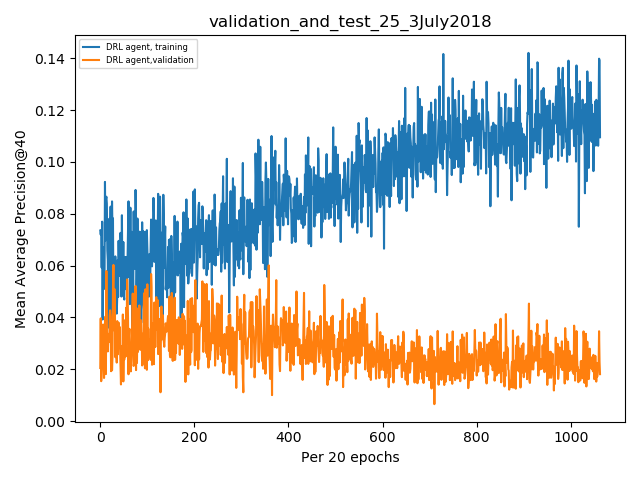
\includegraphics[width=0.8\textwidth]{images/25-25}
	\caption{Training on 25 queries, validating on 25 queries}
	\label{fig:25-25}
\end{figure}


As shown by figure \ref{fig:25-25}, the agent's performance during training improved along with the validation performance for approximately the first 8000 epochs. However, once the training performance begin to show a clear trend upwards, the performance of validation diverged from training performance.  

We experimented with adding more training examples and adjusting the ratio of training and validation queries, hoping this increase in quantity and diversity of topics would lead to better generalization.  To do this we trained on all 50 queries from the previous experiment, and took 10 unseen queries from the WSJ dataset for validation. A similar pattern as the 25-25 split was observed from the result of this variant, as the training performance shows sign of improvement at approximately 8000 epochs, validation performance begin to decreases substantially. This is demonstrated in figure \ref{fig:50-10}.

\begin{figure}[H]
	\centering
	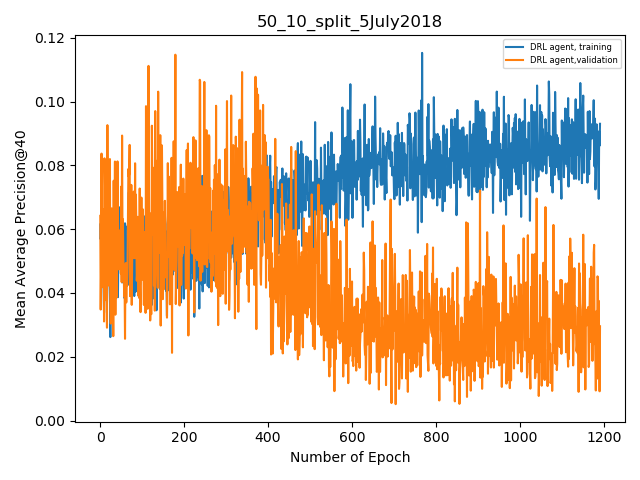
\includegraphics[width=0.8\linewidth]{images/chapter_4/50-10}
	\caption{}
	\label{fig:50-10}
\end{figure}


\subsubsection{Conclusion}

In both variants of this experiment examined, as the performance on the training set showed clear trend of improvement. The validation set showed unstable behaviour, diverging from the training performance.  We wished to gain further insight on the working of the model and investigate the cause of this instability after making this observation.



\subsection{Summary of results, first implementation}

We present the results of both training data and validation data observed from the first implementation in table \ref{tab:MAP_of_splits_sys1}.


\begin{table}[H]
\begin{tabular}{ |p{4cm}||p{3cm}|p{3cm}|p{3cm}|  }
	\hline
	\multicolumn{4}{|c|}{MAP of reformulation compared to baseline} \\
	
	\hline
	                                 & DRL agent                   &baseline(raw ATIRE& improvement from baseline\\
	\hline
		training,25-25    &0.1223                         &0.0864           & $+$0.0359\\
	training ,50-10    & 0.0777                        & 0.0754         & $+$0.0023\\

	\hline
	validation set,25-25 &0.01812                      &  0.08620         &   $-$0.0681         \\
validation set,50-10 & 0.0296                    & 0.0719           & $-$0.0424       \\
	\hline
	
	\end{tabular}
	\caption{\label{tab:MAP_of_splits_sys1}Comparison in MAP between agent's reformulation compared to raw ATIRE search}
\end{table}


\subsubsection{Agent's reformulation behaviour}

Driven by the curiosity to find out what the agent has learnt from training. We compare the reformulated queries against the original queries on a per-query basis, and observe the proportion of the queries that has improved and the queries that has gotten worse after reformulation.



\begin{figure}[H]
	\centering
	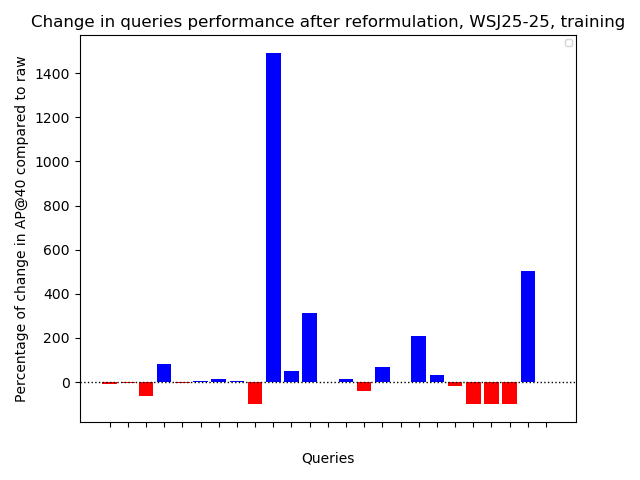
\includegraphics[width=0.7\linewidth]{images/chapter_4/first_system/per_query_improvment/25-25_train}
	\caption{Change in Average Precision on a per query basis, first implementation, 25-25, training set}
	\label{fig:25-25train}
\end{figure}


\begin{figure}[H]
	\centering
	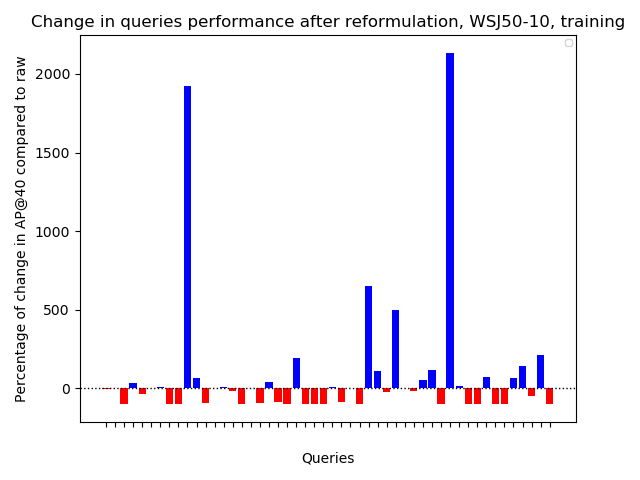
\includegraphics[width=0.7\linewidth]{images/chapter_4/first_system/per_query_improvment/50-10_train}
	\caption{Change in Average Precision on a per query basis, first implementation, 50-10, training set}
	\label{fig:50-10train}
\end{figure}



\begin{figure}[H]
	\centering
	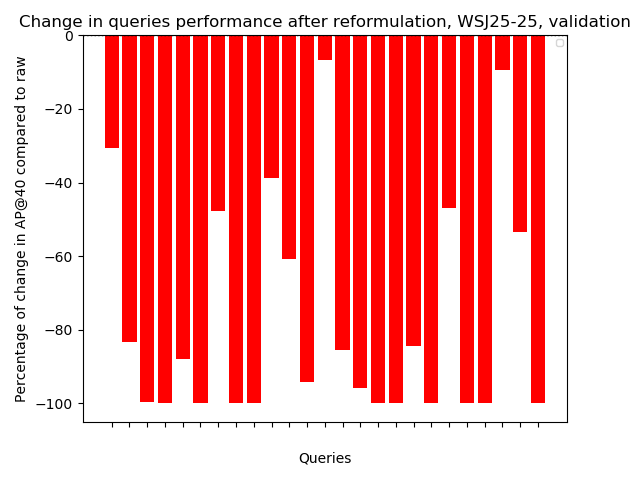
\includegraphics[width=0.7\linewidth]{images/chapter_4/first_system/per_query_improvment/25-25_valid}
	\caption{Change in Average Precision on a per query basis, first implementation, 25-25, validation set}
	\label{fig:25-25valid}
\end{figure}

\begin{figure}[H]
	\centering
	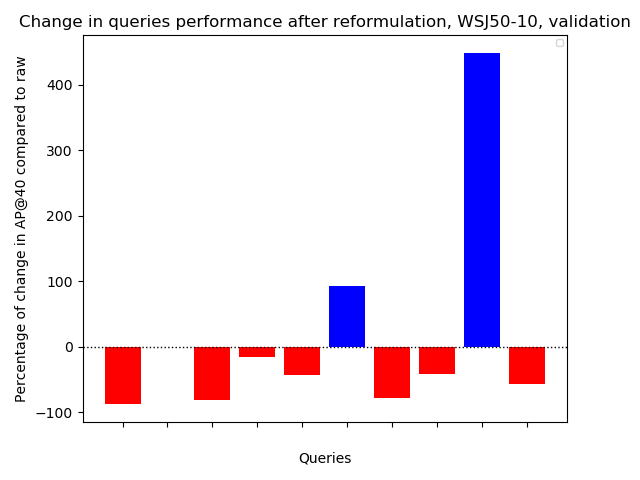
\includegraphics[width=0.7\linewidth]{images/chapter_4/first_system/per_query_improvment/50-10_valid}
	\caption{Change in Average Precision on a per query basis, first implementation, 50-10, training set}
	\label{fig:50-10valid}
\end{figure}


On the training data, we discovered that though overall performance suggested improvement over the raw ATIRE baseline(as shown in table \ref{tab:MAP_of_splits_sys1}), these are the result of a small number of queries which improved substantially, while other queries became worse after reformulation. 

On validation data, we observe that all queries became worse in the 25-25 set, shown in figure \ref{fig:25-25valid}. On the 10 queries used to validate the 50-10 set, two queries improved, 7 became worse, and 1 remained unchanged, we show this in figure \ref{fig:50-10valid}

We examined the output of the agent's reformulation, and found that the reformulated query generated by the agent had a low signal-to-noise ratio, the reformulated queries were long, and consisted of a mix between terms that appeared to be semantically close to the original query, along with terms that appeared to be noise.  We demonstrate several examples in figure \ref{fig:qualitative}

\begin{figure}[H]
	\centering
	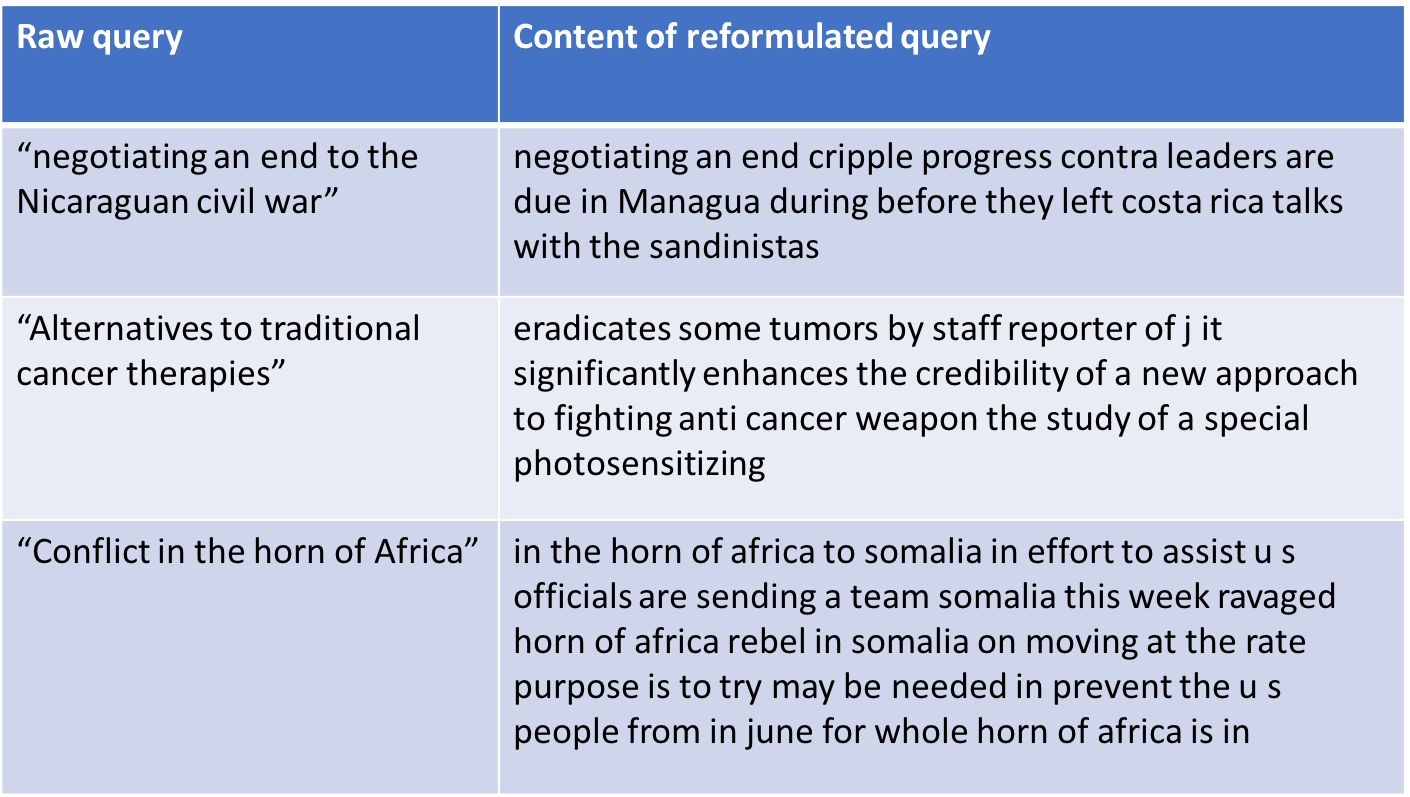
\includegraphics[width=1\linewidth]{images/chapter_4/first_system/per_query_improvment/qualitative}
	\caption{Agent's reformulation}
	\label{fig:qualitative}
\end{figure}


\subsubsection{Conclusion}
As we observe the agent produces very long queries by using all the candidate terms provided, we conclude that the reinforcement learning agent struggled to separate out the useful terms cleanly from noise terms. Perhaps more training examples were needed for the agent to generalize more effectively. 



\subsection{Failed attempt to scale up training data}

Speculating the agent would both learn and generalize better if more training examples are provided, in this experiment we attempted to scale up the size of the training data. We took 1000 queries from the MSA dataset,  training on 800, and validate on 200 queries. 

\subsubsection{Results}

Training on this larger dataset took a longer time frame than what is practical. Completing a single epoch through the training data took over one day. This made it impractical to train on data of such scale. We were unable to get meaning results from this experiment due to this scalability issue.





%
%\begin{figure}[H]
%  \centering
%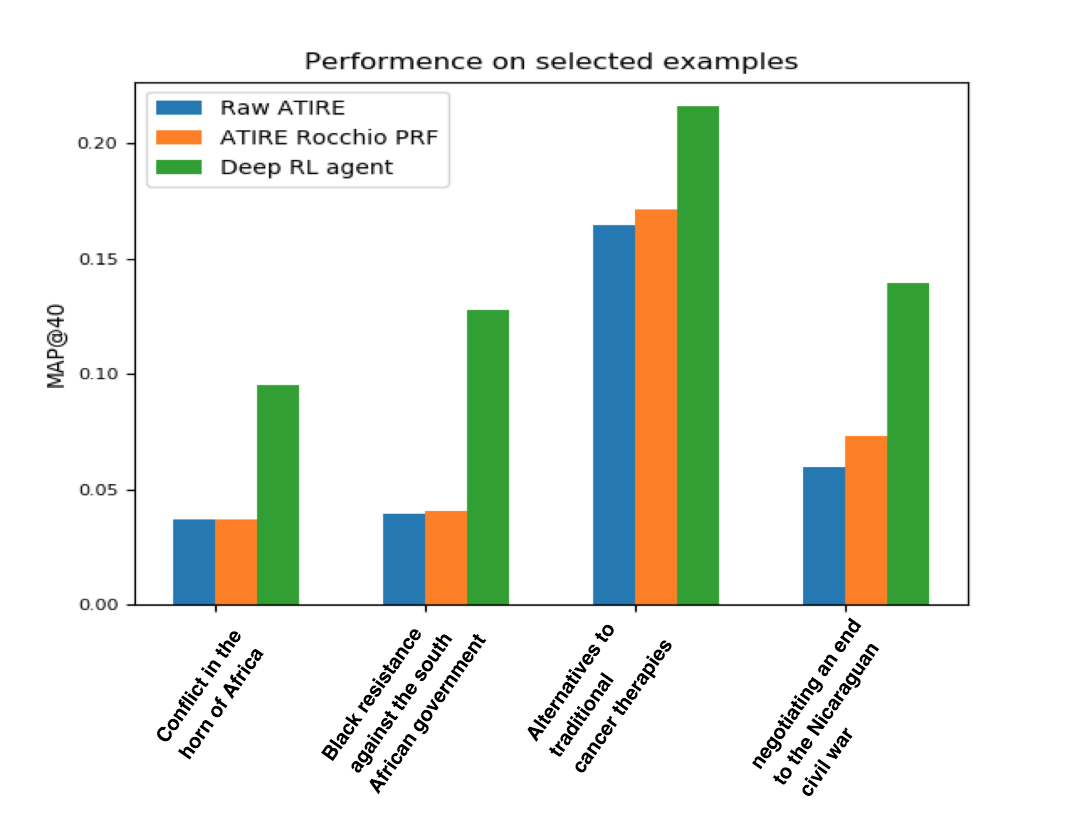
\includegraphics[width=1\textwidth]{images/chapter_4/Chapter_4-bar_graph.png}
%  \caption{}
%    \label{fig:bargraph}
%\end{figure}

%
%
%
%We demonstrate this comparison in figure \ref{fig:bargraph}. In these queries, the agent’s reformulation led to an increase of average precision compared to the baseline score, in some cases, more than double the baseline values. However, such occurrences were rare. The majority of the queries performed worse than the baselines. 
%
%A similar observation was made in the reformulation of set of queries used for training. We found that though some improvement occurred in the training sets, these are the result of extremely high performance from a small number of queries. The rest either remained similar to baseline, or worsened. 




\subsubsection{Experiments summary}

At this point we had achieved the task of building a deep reinforcement learning based framework for query reformulation based closely on the descriptions provided in the paper by Nogueira \& Cho\cite{nogueira2017task}, though it was not producing comparable results to theirs. As we attempt to scale up the data size, we encountered scalability issues, which must be mitigated if we were to investigate the effect of training on a larger quantity of data.



\subsection{Issues revealed by experiments}


It is important to understand the issues and obstacles facing this implementation to looks for points of improvement. Perhaps the biggest issue we faced during this implementation was understanding how this problem lend itself to the framework of a reinforcement learning problem. This was first observed as we construct the theoretical model in the previous chapter, we hoped this would become apparent during the implementation process, but this was not the case.

Firstly, there is a level of unresolved ambiguity over how this problem would be posed as a reinforcement learning problem. In a typical reinforcement learning problem (demonstrated in figure \ref{fig:agent-environment}), at each time step the agent send an action to the environment, and receives a state, action, reward, and the next state after the action has been taken from the environment. This two-way interaction between the agent and the environment is crucial for the agent to learn the dynamics of the environment and improve the policy parameters towards a desirable direction. 

In query reformulation, the notion of state can be interpreted in a multiple ways.  Nogueira \& Cho\cite{nogueira2017task} implies that the agent only sees one candidate term at a time and make one decision on whether or not to include the term in a reformulated query, as illustrated previously in Figure \ref{fig:CNN1}.  Thus the state can either be interpreted as the original query to be reformulated, the combination of the original query and the current candidate term, or the entire set of retrieved candidate documents. 

Just as the state can have open interpretation, we can interpret action in several ways. The action can be viewed as each binary decision to include a candidate term, based on the raw term and the query. 

This interpretation makes the problem episodic, where the reward is treated as latent until the end of the episode. The next state is the next candidate term available. Reward is 0 until the entire reformulated query is sent to the search engine for scoring. A comparable example to this interpretation would be a game of pong, where each state is the current image demonstrating the ball's location, the action choices are to move the paddle up or down, and no reward is given until a game is either won or lost.  From the paper's description this is heavily implied. 

Equally, from another perspective, this problem could be viewed as sending only one action to the environment, since only one reward is receivable after the reformulated query has been sent to the search engine. In this case, the action is a binary vector the same size as the candidate terms set. In this case, the notion of “next state” does not exist in the problem of query reformulation, because query reformulation is one shot.

Another issue we observe is that the agent cannot effectively handle a large action space. As the size of the candidate term set increases, the agent becomes both ineffective and inefficient.  As a result, this implementation has a impractically long training time on non trivial data size. This is a major obstacle which prevents us from training on larger datasets, making it difficult to verify whether the agent’s suboptimal performance is due to a lack of training examples, poor choice of hyper parameters, or the architecture of the model itself. Furthermore, we observe a difficulty for the agent to separate out useful terms from noise when more than a trivial number of terms are presented for picking. 



\subsubsection{Summary of conclusions reached from first implementation}


We conclude that either we misinterpreted some critical details in the paper, or there are details important to performance that is not documented in the paper. We set out to gather additional information from various sources to supplement our understanding of the framework.

During this period, we also made a series of adjustments to the model with the aim of improving performance on the small dataset, these include changing the size of the network, experiment with different learning rates, and term embedding parameters. However, none of these adjustments made significant impact on the agent’s performance so we will not present them in detail.


%%%%%%%%%%%%%%%%%%%%%%%%%%%%%%%%%%%%%%%%%%%%%%%%%%%%%%%%%%%%%%%%%%%%%%%%%%%%%%%%%%%%%%%%%%%%%%%%%%%%%%%%%%%%%%%%%%%%%%%%%%%%%%%%%%%%%%%%%%%%%%%%%%%%%%%%%%%%%%%%%



\section{Gathering additional information}

We contacted the principal author, Nogueira, enquiring for clarification in regards to our questions on the nature of the problem, as well as any important details not included in the original paper. From our correspondence with Nogueira we acquired several insights and heuristics which were not included in the original paper. Nogueira expressed those were crucial in building the system. Many of which would make the difference between the agent learning and failing completely. 


\subsection{Clarification on how the problem is framed}

In our correspondence with Nogueira, a clarification of the problem’s framing was provided. Nogueira confirms that action in this problem is a single, albeit highly complex action.  The action for each query is, in essence, a single bit vector with length $N$, where N is the size of the candidate terms set. Each element of the vector contains a binary decision to include or exclude the corresponding candidate term in the reformulated query. This makes the action space size $2^{N}$.

There were mixed statements about what is the state should be in this problem. Nogueira suggested that one way to frame this problem is as a bandit problem, a special case of a reinforcement problem where the notion of state is not used. The other way to frame this is as a single state reinforcement learning problem, where the original query and the list of documents retrieved in the first round is treated as the state.

Both interpretations has elements which makes it slightly awkward to fit a query reformulation problem to. Bandit problems are a well studied class of problems in literature where algorithms used is different from a standard reinforcement learning. There are no mentioning of this in the original paper by Nogueira \& Cho\cite{nogueira2017task}. Furthermore, the state is used by the value network to predict the expected reward, $\bar{R}$. 

For these reasons, we choose to interpret the problem as a reinforcement learning problem with single state, where the number of available actions are astronomically large, scaling exponentially with the size of the input.  As only a subset of the documents retrieved is used as candidate terms set for reformulation, we view the state as partially observable. 

\subsection{Additional implementation details}

Aside from clarifying the framing of the problem, several implementation details were provided by Nogueira in our correspondence. These were not included in the published paper. 

\subsubsection{Inclusion of the raw query}

The most important detail we received from Nogueira was to always include the original raw query, $q_0$, in the reformulated query.  If none of the candidate terms are selected, $q_0$ is still sent to the search engine for scoring.  This seemed like a minor detail, but we found this resulted in substantial improvement to the reformulated query's score. With this adjustment the value predictor can learn the value of  $q_0$ quickly, which is the score if the agent selected no additional terms. 

This has several implications. Firstly, always including $q_0$ means the agent is less likely to perform worse than the raw search baseline, unless the agent stumble across an unusually bad policy. As we had shown in previous experiments the agent can travel towards the direction of positive rewards, we expect such occurrences to be rare. 

Including the raw query in scoring also provides a baseline value estimator to learn. The means the agent would be sensitive to any changes to the reward as a result of actions taken. As defined by the cost function of the policy agent, the learning mechanism relies on the dynamic between the value estimator and the policy generator. Performing worse than expected will lead to negative rewards which makes the actions less likely to occur in the future.

\subsubsection{Adding a manual bias}

Nogueira also suggested that we manually bias the output of the policy network, such that the output is likely to output 0 in most of the cases, leading to the agent selecting no terms from the candidate terms set. Nogueira suggested initializing the bias value before the final output to an extremely large value, such as 10.0. In deep neural networks, bias is usually set to a small value such as 0.01. Using an unusually large value makes it extremely rare for the agent to actually pick a new term from the candidate term for reformulation. 
 
Nogueira explained that this step is important as it allows the value network to learn the reward produced by only the original query at first, and so the agent would be sensitive to any change in reward. This would force the value network's output l into a reasonably accurate range before policy training begins. Thus any updates on the policy estimator’s parameters would be following the gradient in the right direction. Nogueira mentioned that without this step the agent ``does not learn anything” for over 2 weeks in their experiments.   

\subsubsection{Additional information on Convolutional Neural Network architecture}
%\todo{Review this section}

It was also revealed that our previous interpretation of using a sliding window to capture the context term was incorrect. Nogueira explained that all candidate terms, in their word2vec embedded form, are fed to the agent at once. Our previous interpretation of feeding in a single candidate term with a number of context term on each side of it was different from what Nogueira intended. Under this new interpretation, input of each raw query is a matrix of number of candidate terms $\times$ dimension of word embeddings. The ``context window'' is the width of the filter in the convolution layers in the CNN. 

\todo{This may need better explanation, maybe a diagram?}

%We foundenquired whether using hierarchical CNN was the correct approach for this problem, Nogueira 


\section{Re-implementation of the system(In progress)}

Incorporating the additional information acquired from Nogueira, we reimplemented our reformulation system with these changes:


\subsection{Including the raw query}
We now append the raw query, $q_0$, to the terms chosen by the agent for reformulation. In the case where the agent does not choose any term, we pass $q_0$ to the search engine for scoring regardless. This should ensure that the value network learns the value of $q_0$ when no candidate term is selected for reformulation.
\subsection{Candidate terms and capturing context}
The entire set of candidate terms are now fed into the system in one lot, instead of moving a sliding window as illustrated by figure \ref{fig:chapter4-contextwindow}. 
\subsection{Experimenting with an alternative approach to CNN}

\todo{Why?}
\todo{How is it different to Hierarchical CNN}
\todo{What was the effect of this?}


\section{Experiments}


\subsection{Experiment configurations}
\subsubsection{Source of candidate terms}

We saw from the previous experiments that having a large action space led to scalability problems. 

From the first round of retrieval, we take the first 200 terms from a single document sampled uniformly from the top 10 documents in the results list as a source of candidate terms. This is because the average length of a paragraph is approximately 200 words, and we expect that a document should cover the main topics which the document is about within the first paragraph. Sampling from the top 10 documents for reformulation is a trade off between 


\subsubsection{Data sets}

From the WSJ dataset, we used a training and validation split of 25-25 and 50-10. These are the same splits from the previous series of experiments, we do so to compare the effect of the second implementation compared to the first.

In later experiments, as we wished to train the agent with even more training examples to observe the effect of increased training examples on generalization. We took queries from the WSJ dataset, training on 100 queries and validating on 25 queries. This is the 100-25 split.

For a more scaled up experiment, we took 800 queries from the MSA dataset for training, while validating on 200 queries. 


\subsubsection{Metrics and baselines}
Similar to previous experiments, MAP@40 is used to evaluate the reformulated queries.

\subsubsection{Hyper parameters}
We used the following hype hyper parameters during this experiment.

\begin{itemize}
	\item ADAM Optimizer, with the same parameter as last implementation.
	\item 512 neurons in the fully connected layers.
	\item CNN window size of 9 and 3, using 256 filters.
\end{itemize}





\subsection{Effect of making changes to the system(In progress)}


\subsubsection{Using non hierarchical convolution neural network}

We observe a faster training time by eliminating the step where we using a sliding window approach to break inputs down into a single candidate term surrounded by a number of context terms. 

\subsubsection{Effect of including the raw query}
As we expected, always including the raw query along with terms chosen by the agent during the scoring process led to substantial improvement in the training performance. The performance on the training data also exhibits a clear trend to converge. 

\subsubsection{Effect of manually biasing to the network}

Nogueira maintained that it is important to manually bias the policy network such that term selection would be rare. Surprisingly, we found this approach to be  ineffective. An agent trained in this fashion does not exhibit signs of learning. We train on WSJ100-25 set, and present the training performance in figure \ref{fig:largebias}.


\begin{figure}[H]
	\centering
	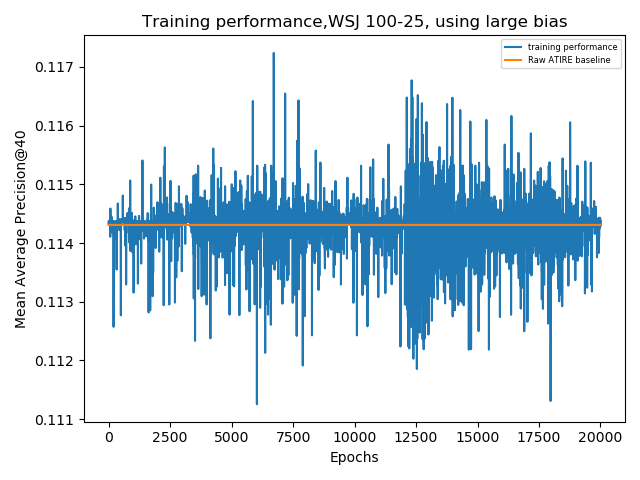
\includegraphics[width=0.7\linewidth]{images/chapter_4/second_system/large_bias}
	\caption{Using a bias of 10.0}
	\label{fig:largebias}
\end{figure}



\subsubsection{Conclusion}
We decided to disregard the advice to manually bias the policy network, while incorporating the other changes into our experiments.

\subsection{Agent performance on training data}

We wished to evaluate the performance of the system on training data to confirm that the agent is capable of training well on a variety of data size, in a reasonable time frame. We define reasonable time frame for a single experiment duration measured in days, instead of weeks. 
We train the agent on 4 datasets of various size until convergence, and observe it's performance compared to raw ATIRE search baseline.

\subsubsection{Results}

We first trained the agent on 25 queries, the same dataset used in the previous series of experiments. The result is shown in figure \ref{fig:training2525}. 

\begin{figure}[H]
	\centering
	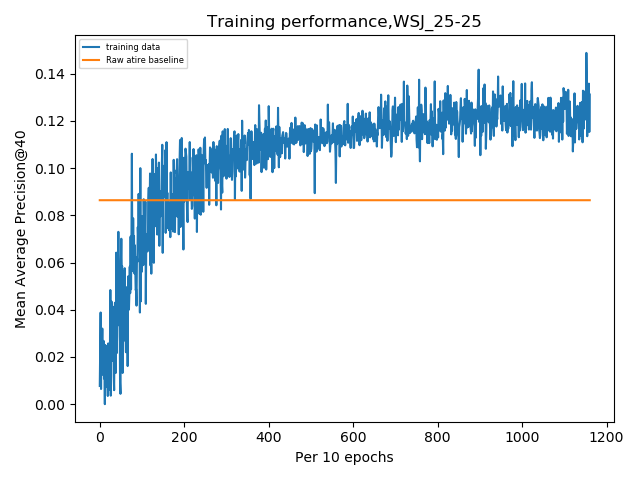
\includegraphics[width=0.7\linewidth]{images/chapter_4/second_system/training_2525}
	\caption{}
	\label{fig:training2525}
\end{figure}

Next, we trained on 50 queries, the results are shown in \ref{fig:training5010}.

\begin{figure}[H]
	\centering
	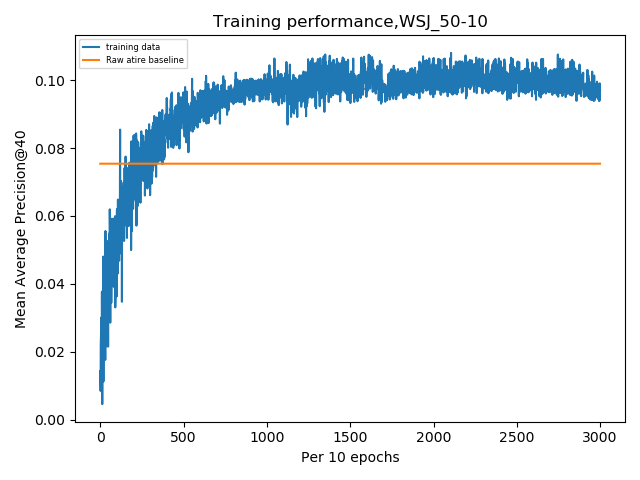
\includegraphics[width=0.7\linewidth]{images/chapter_4/second_system/training_5010}
	\caption{}
	\label{fig:training5010}
\end{figure}

Stepping up the size of the training set, we train the system using 100 queries, the results are shown in figure \ref{fig:training10010}


\begin{figure}[H]
	\centering
	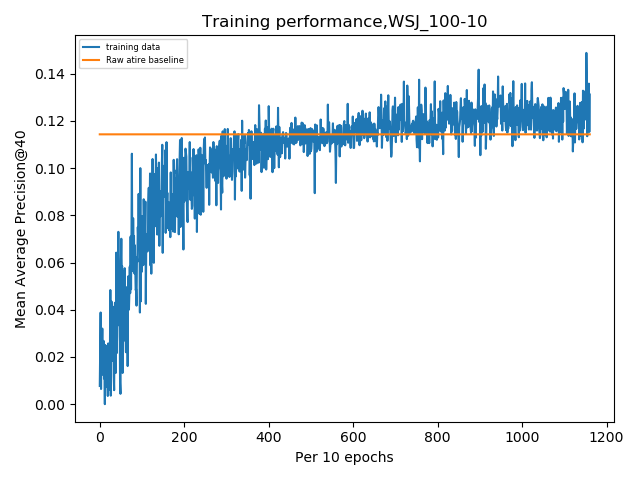
\includegraphics[width=0.7\linewidth]{images/chapter_4/second_system/training_10010}
	\caption{}
	\label{fig:training10010}
\end{figure}

Finally, we used the MSA dataset that was previous too large for the system to handle in a reasonable time frame. There are 800 training queries in this dataset, the results are presented in \ref{fig:trainingmsa}

\begin{figure}[H]
	\centering
	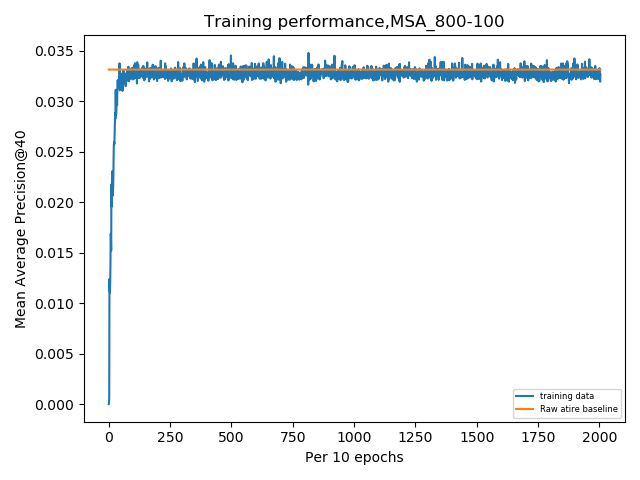
\includegraphics[width=0.7\linewidth]{images/chapter_4/second_system/training_msa}
	\caption{}
	\label{fig:trainingmsa}
\end{figure}




\subsubsection{Conclusion}

In all 4 experiments, the agent's training performance converged, performing at least as good as raw ATIRE in Mean Average Precision. We conclude that this is a result of appending the raw query to the reformulated query for scoring. The agent is unlikely to perform worse than the raw baseline. 

\subsection{Training performance compared to generalization}
We investigated the relationship between learning and generalization by letting the agent reformulate an unseen set of validation queries after every 10 epochs of training. In this section we report our findings.

\subsubsection{Results}

We used the same 25-25 split from the previous series of experiments and ran them through the updated reformulation system. As we expected, despite convergence on training data,  little improvement in validation occurred as there are too few training examples. We stopped the training at 12000 epochs, after the training performance has already converged for many epochs, and validation performance showed little improvement. The result is shown in figure \ref{fig:trainvsvalid25-25}

\begin{figure}[H]
	\centering
	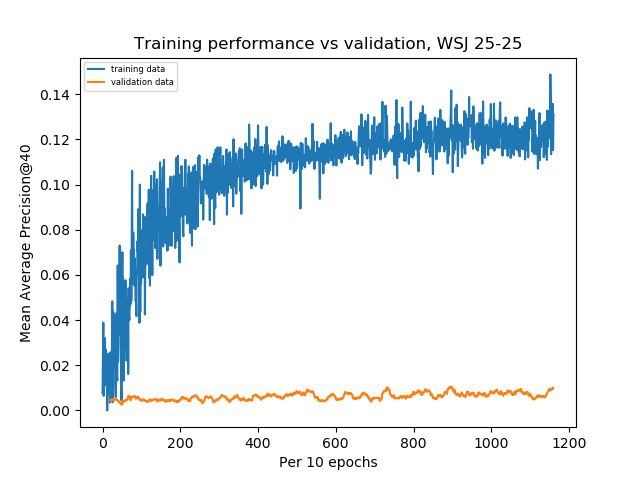
\includegraphics[width=0.7\linewidth]{images/chapter_4/second_system/train_vs_valid_25-25}
	\caption{}
	\label{fig:trainvsvalid25-25}
\end{figure}

Next, we trained on 50 queries and validated on 10 queries, during this experiment we let the agent train for longer than the previous experiment. We observe that between epochs 0 and 10,000 there are no clear trends in the performance on the validate set of queries, though convergence occurs on the training set. Between epochs 10,000 and 15,000 the performance on the validation set begins to show clear sign of improvement. We continue to train the agent, finishing at 30,000 epochs. The results are presented in figure \ref{fig:trainvsvalid50-10}. 


\begin{figure}[H]
	\centering
	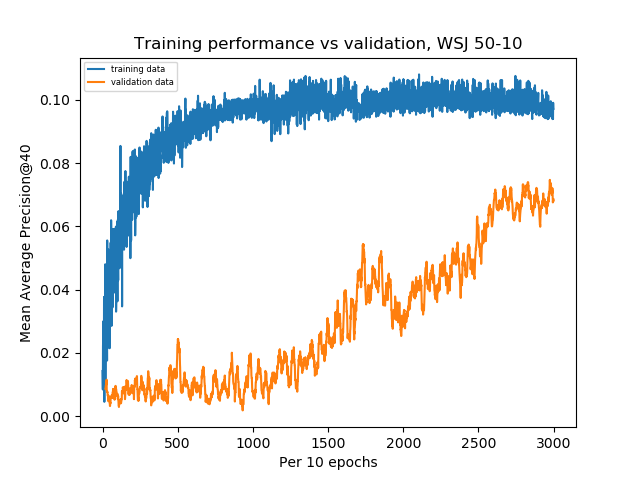
\includegraphics[width=0.7\linewidth]{images/chapter_4/second_system/train_vs_valid_50-10}
	\caption{}
	\label{fig:trainvsvalid50-10}
\end{figure}

On our third WSJ data set, we train on 100 queries, and validate on 25 unseen queries for 30,000 epochs, the result is shown in figure \ref{fig:trainvsvalid100-25}. 

\begin{figure}[H]
	\centering
	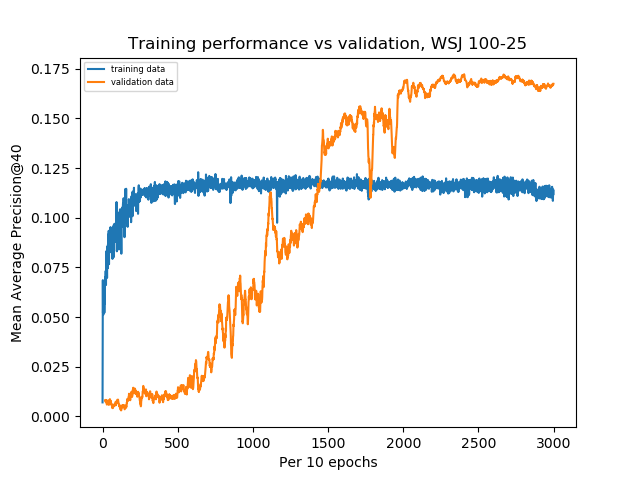
\includegraphics[width=0.7\linewidth]{images/chapter_4/second_system/train_vs_valid_100-25}
	\caption{}
	\label{fig:trainvsvalid100-25}
\end{figure}

We then investigate how well the agent would generalize to unseen queries on a different task, we training the agent on 800 queries from the MSA dataset, and validate on 100. We present the result in figure \ref{fig:trainvsvalid800-100}. We observe an increase in validation performance at around epoch 3500. Then it appears that it is reached convergence, as it ceases to show signs of improvement. We stopped this experiment at epoch 20,000.

\begin{figure}[H]
	\centering
	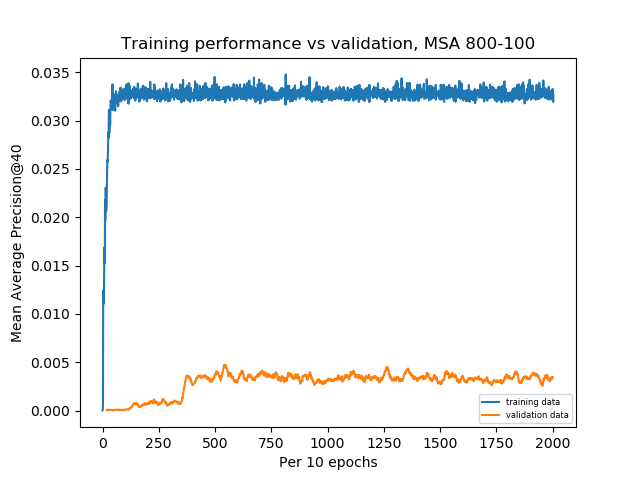
\includegraphics[width=0.7\linewidth]{images/chapter_4/second_system/train_vs_valid_800-100}
	\caption{}
	\label{fig:trainvsvalid800-100}
\end{figure}





\subsubsection{Conclusion}

We conclude that the agent is capable of learning to reformulate a set of queries, and capable of generalizing to unseen examples if the set of training queries are large enough in numbers, and cover diverse topics. Clearly, the agent is unlikely to generalize effectively when training examples are few and the topics are not diverse, as is the case with WSJ25-25. 

It is interesting to observe that though the performance appears to have converged on the training set, improvement in the validation queries may not occur for many epochs, during this period there is no substantial change in the performance of the agent on the training set. Simply monitoring the training performance may suggest that the agent has stopped learning. However, after the agent's performance has converged on the training set, it continues to improve on the validation set, sometimes substantially.





\subsection{Instability with different random seed}

During our experiments we observe that the agent exhibited a strange, unstable behaviour. We found that several identically set up experiment (same code, same data) will exhibit very different performance and results dependent when a different pseudo random seed is used for initialization of the neural network model. We decided to investigate this phenomenon systematically 


\subsubsection{Results}

We trained the agent on 50 queries for 5000 epochs, with identical code and hyperparameters, but used a different random seed to initialize the system. We then observed the training performance,  presented in figure \ref{fig:trainvsvalid50-10badseed}. 

On one of the three seeds, the agent's performance clearly move towards convergence. However, on the other two seeds, there is no clear trend upwards. The agent fails to reach any substantial reward, and even gradually moves downwards towards 0 over time. This is a concerning observation. As we observed previously that always including the raw query means that the agent is unlikely to perform worse than raw on any reasonable, when the agent exhibit this type of behaviour it indicates that no training occurred, and is highly unlikely that learning will happen eventually in these circumstances. 



\begin{figure}[H]
	\centering
	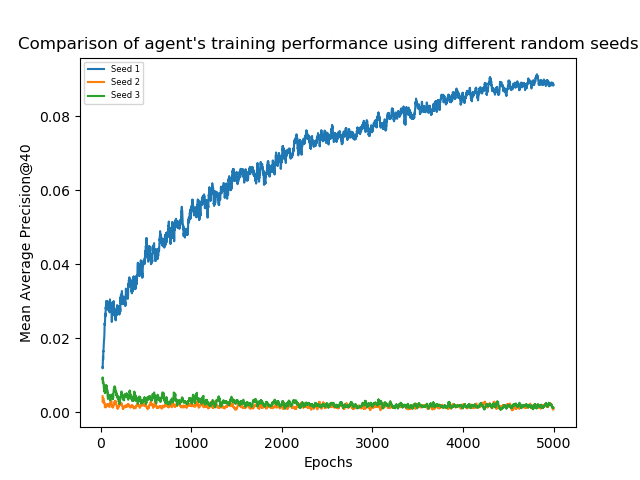
\includegraphics[width=0.7\linewidth]{images/chapter_4/second_system/seed_comparision}
	\caption{}
	\label{fig:seedcomparision}
\end{figure}


We observed the trend between learning and generalization on a poorly initialized run to see if any generalization is built at all, this observation is presented in figure \ref{fig:trainvsvalid50-10badseed}. As we expected, a run with a bad random seed resulted in the agent neither learning the training examples, or form any clear generalization. 


 \begin{figure}[H]
 	\centering
 	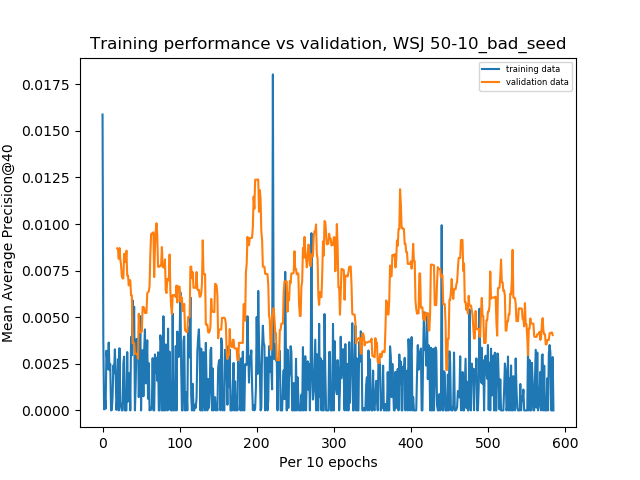
\includegraphics[width=0.7\linewidth]{images/chapter_4/second_system/train_vs_valid_50-10_bad_seed}
 	\caption{}
 	\label{fig:trainvsvalid50-10badseed}
 \end{figure}



\subsubsection{Conclusion}


This is a concerning observation which appears to be an innate drawback to deep reinforcement learning. We found several cases in literature reporting similar behaviour. \cite{rlblogpost}

The instability of deep reinforcement learning makes experimentation and reporting difficult. When an experiment fails to perform as we expected, it is not possible to tell whether it is due to an error in the implementation, poor parameter choice, poor data balance, or simple a case of poor initialization. Before we discovered that simple varying the random seed may result in such substantial difference in performance, many hours were spent in debugging and experimenting with various model configurations. This made experimentation time consuming, and it is sometimes possible to disregard a good model configuration simply because of ``unluckiness'' in initialization, as we found out that an implementation which works well can suffer substantially from simply changing the random seed.

Likewise, when the agent performs well, we are unable to be certain that it is the best outcome we can achieve, or whether there are better results achievable by using a different model configuration, changing hyper parameters, or simply changing the random initialization. As there are an infinite number of random seeds we could use, and it is not practical to run through a large number of them once the size of the training data becomes non-trivial. It also would not make sense to take the mean value, as many random seeds leads to complete failure in the system. For the purpose of this thesis, we will the best results we have seen thus far.
 




\subsection{Summary of results}



\subsubsection{Repeating experiments from first implementation}

\begin{table}[H]
	
	\begin{tabular}{ |p{4cm}||p{3cm}|p{3cm}|p{3cm}|  }
		\hline
		\multicolumn{4}{|c|}{MAP of reformulation compared to baseline} \\
		
		\hline
		& DRL agent, 2nd implementation               &baseline(raw ATIRE)& improvement from baseline\\
		\hline
		training,WSJ25-25    &0.1335                        &0.0864           & $+$0.0471\\
		training ,WSJ50-10    & 0.0987                       & 0.0754         & $+$0.0233\\
		
		\hline
		validation ,WSJ25-25 &0.0138                       &  0.0862           &$-$0.0723           \\
		validation ,WSJ50-10 & 0.0747                      & 0.0719           & $+$ 0.0028     \\
		\hline
	\end{tabular}
	\caption{\label{tab:MAP_of_splits_small}Comparison in MAP between agent's reformulation compared to raw ATIRE search}
\end{table}





\subsubsection{New experiments in second implementation}

We present the results from training on two larger sets of queries in \ref{tab:MAP_of_splits_sys2}. 


\begin{table}[H]
	
	\begin{tabular}{ |p{4cm}||p{3cm}|p{3cm}|p{3cm}|  }
		\hline
		\multicolumn{4}{|c|}{MAP of reformulation compared to baseline} \\
		
		\hline
		& DRL agent, 2nd implementation               &baseline(raw ATIRE)& improvement from baseline\\
		\hline
		training,WSJ100-25    	&0.1155                       &0.1143         & $+$0.0011\\
		training,MSA800-200    &0.0335                       &0.0327       	& $+$0.0008\\
		
		\hline
		validation,WSJ100-25  	&0.1695                    	 & 0.1667         &$+$0.0028\\
		validation,MSA800-200 &0.0077                   	 &0.0311        & $-$0.0234 \\
		\hline
	\end{tabular}
	\caption{\label{tab:MAP_of_splits_sys2}Agent's performance on larger data size compared to raw ATIRE}
\end{table}


We conducted a paired t-test against the null hypothesis that reformulation made no difference to the MAP of these sets of queries. The $p$-value suggests that these differences are considered statistically insignificant. 



\subsection{Discussions}


\subsubsection{Improved training speed}
Changing the  larger datasets and train in a more reasonable time frame, training an agent for 30,000 epochs on 800 training queries now take less than a week. In the previous implementation, a single epoch took over one day to complete. This is very useful as it allows us to conduct more experiments in a given time period. This is crucial as Deep Reinforcement Learning experiments can take many epochs to train, and many trial and error is required when the agent fails to perform.



\subsubsection{No-op problem}

Examining the individual queries and our paired t-test results suggests that improvement observed is not statistically significant. We observe that the agent collapses into a policy of taking no action for many queries. We demonstrate this phenomenon in figure \ref{fig:100-25train}  and figure \ref{fig:100-25valid}, showing the per query change in scoring in WSJ100-25 for training and validation, respectively.  

\begin{figure}[H]
	\centering
	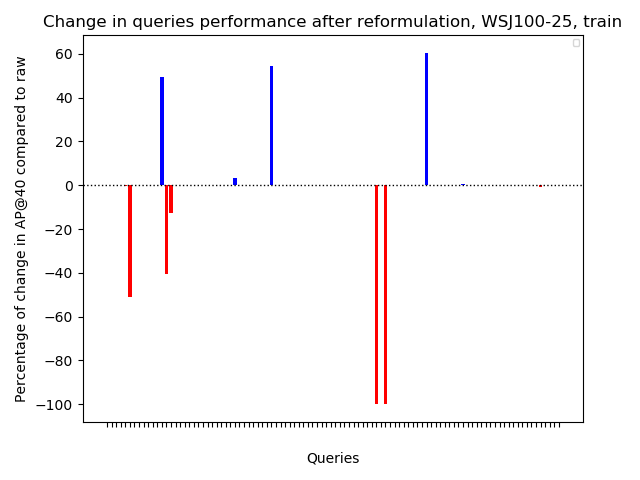
\includegraphics[width=0.7\linewidth]{images/chapter_4/second_system/100-25_train}
	\caption{}
	\label{fig:100-25train}
\end{figure}


\begin{figure}[H]
	\centering
	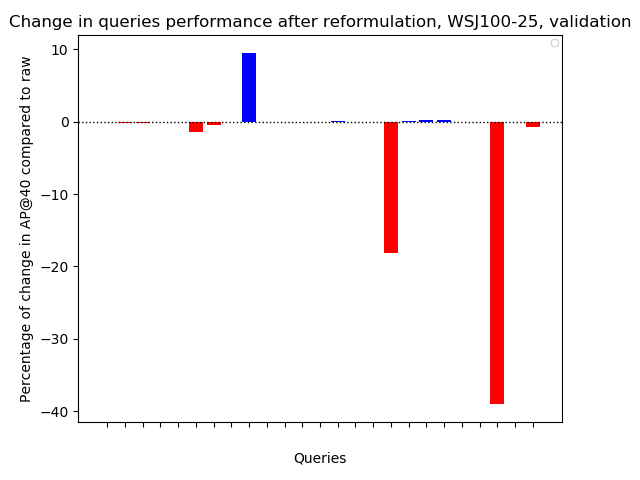
\includegraphics[width=0.7\linewidth]{images/chapter_4/second_system/100-25_valid}
	\caption{}
	\label{fig:100-25valid}
\end{figure}



\subsubsection{Challenges in reproducing Deep Reinforcement Learning experiments}

Reproducing the work of Nogueira \& Cho was not a trivial process as we had initially expected. During this process we found that there are many challenges to this pursuit, including misinterpretation of details provided, and incomplete description in published work. Even a working system can be highly unstable, where changing the random seed in a working system can result in complete failure.

It appears that is not a unique problem to us. Henderson et al,.\cite{henderson2017deep} conducted a study on the reproducibility of deep reinforcement learning based experiments, and highlighted the unstable nature of reinforcement learning through several findings. Henderson et al,. reported that different implementation of the same algorithms, on the same task, using the same hyper-parameters resulted in substantially different performance. Other factors that can change the the system's performance substantially are multiplying the reward by a constant, and using different random seeds to initialize. 

Combining these findings and our own experience, we question whether it is actually possible to reproduce a deep reinforcement learning experiment and get the same results by following a description provided.









\section{Chapter summary}


This chapter documents the reproduction of the query reformulation system based on the framework of Nogueira \& Cho\cite{nogueira2017task}. The first implementation of the system was based on our interpretation the descriptions provided in the paper, which works on trivial problems, but fail to perform as the size of the input data grow. 

We contacted Nogueira, the principal author behind the framework additional information which was not included in the paper in order to improve the system's performance. The additional information proved very important. Incorporating this information into our implementation improved the reformulator's performance substantially, both in efficiency and effectiveness from the previous implementation. Although the results of this implementation did not show significant improvement over the baseline, the new insights allowed us to develop further intuition about the problem. These details highlight the importance of getting the value estimator into a relatively accurate range. We use this knowledge to devise a training scheme with the goal of improving the performance of the agent in the next chapter. 


